%%%%%%%%%%%%%%%%%%%%%%%%%%%%%%%%%%%%%%%%%%%%%%%%%%%%%%%%
%%%%                                              %%%%%%
%%%%  Author: Peter Wilson                        %%%%%%
%%%%                                              %%%%%%
%%%%  ANDES quad element                          %%%%%%
%%%%                                              %%%%%%
%%%%%%%%%%%%%%%%%%%%%%%%%%%%%%%%%%%%%%%%%%%%%%%%%%%%%%%%


%fref generates automatically the respective abreviation/word in the text for the reference. You just have to define a label starting with the respective keyword.
%english: chap, sec, fig, eq, app
%deutsch: chap/kap, abs, abb, gl, anh
%see http://ctan.space-pro.be/tex-archive/macros/latex/contrib/fancyref/fancyref.pdf for more information

\renewcommand{\Thema}{Benchmarking}



\chapter{Benchmarking}

Benchmarking yeah

\section{Static benchmarks: shell obstacle course}

To test the correct derivation and implementation of the thin quad shell element, the shell obstacle course proposed by Belytschko \cite{Bel85} is considered.

\subsection{Scordelis-Lo roof}

\begin{wrapfigure}{r}{0.45\textwidth}
	\centering
	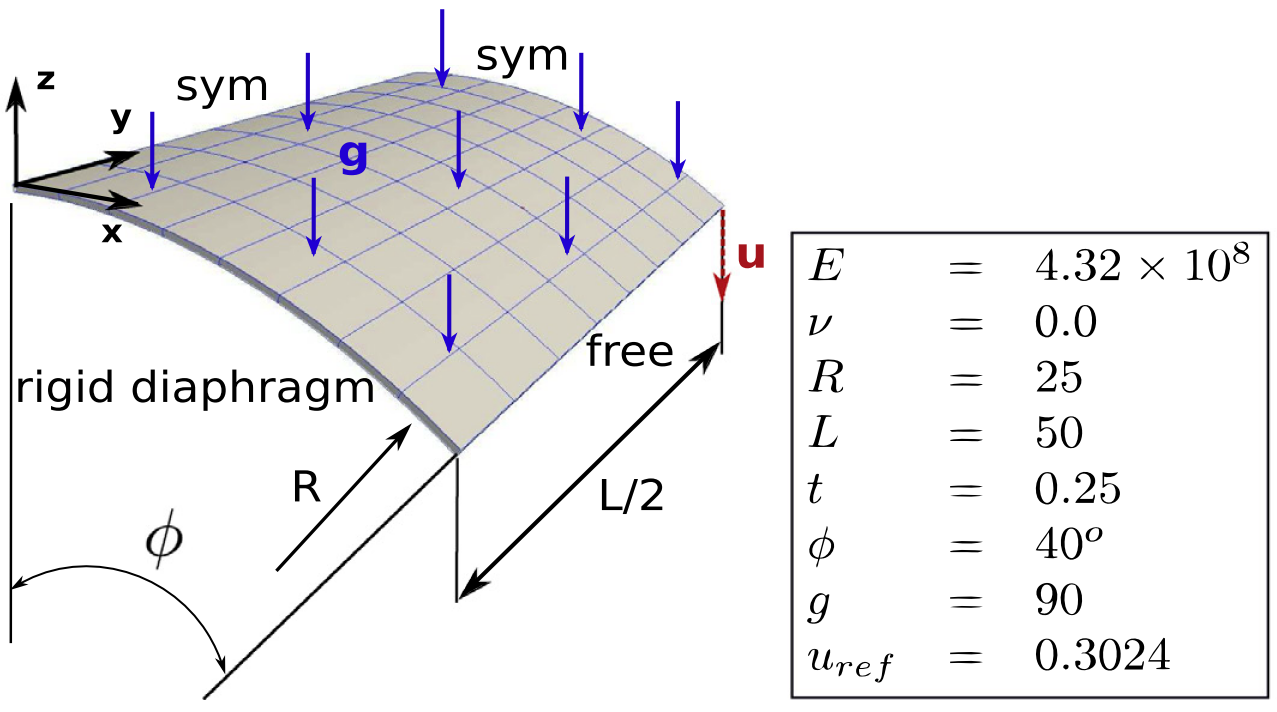
\includegraphics[width=0.40\textwidth]{images/scordelisroof.png}
	\caption{Definition of the Scordelis-Lo roof benchmark\cite{Bou13}}
\end{wrapfigure}

The Scordelis-Lo roof is part of a cylindrical shell fixed by rigid diaphragms at it's axial ends. The only loading is a pseudo-gravity distributed load that has a magnitude of 90. Due to symmetry only a quarter of the shell is modelled. The key result is the vertical displacement of the lateral side at the midpoint, denoted by $\textcolor{red}{u}$ in the following diagram. The reference value is $u_{ref} = 0.3024$.



 
\begin{figure}[H]
	\subfloat[Quadrilateral element convergence for the Scordelis-Lo roof benchmark]
	{\label{ref_label2}
		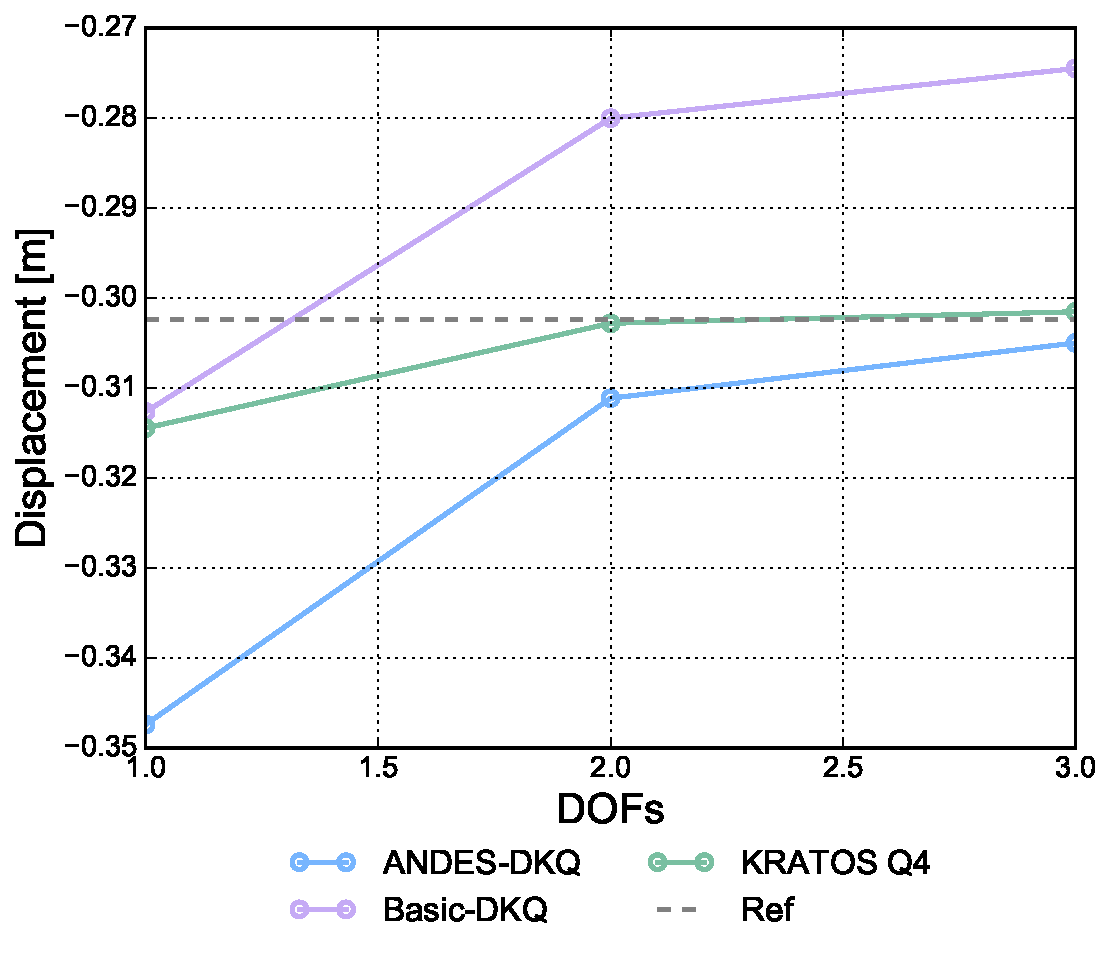
\includegraphics[width=7.3cm]
		{scordelis_structured_quad_results.pdf}}
	\subfloat[Triangle element convergence for the Scordelis-Lo roof benchmark]
	{\label{ref_label2}
		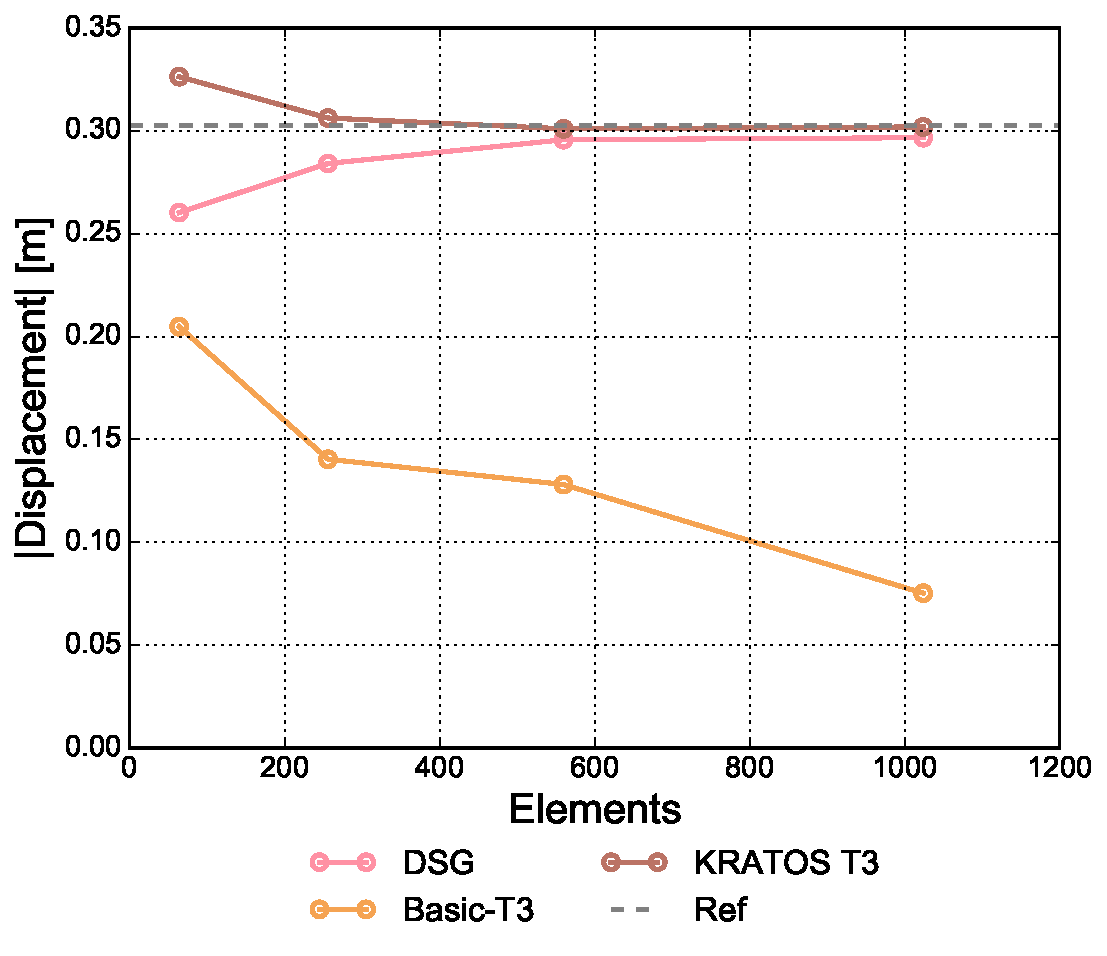
\includegraphics[width=7.3cm]
		{scordelis_structured_tri_results.pdf}}
	\caption{\label{ref_label_overall}Scordelis-Lo roof benchmark results}
\end{figure}

 

Fixup tri results

The performance of the element is demonstrated in the convergence graph above. It is clear that the element agrees with the reference solution.

\subsection{Pinched cylinder}

\begin{wrapfigure}{r}{0.45\textwidth}
	\centering
	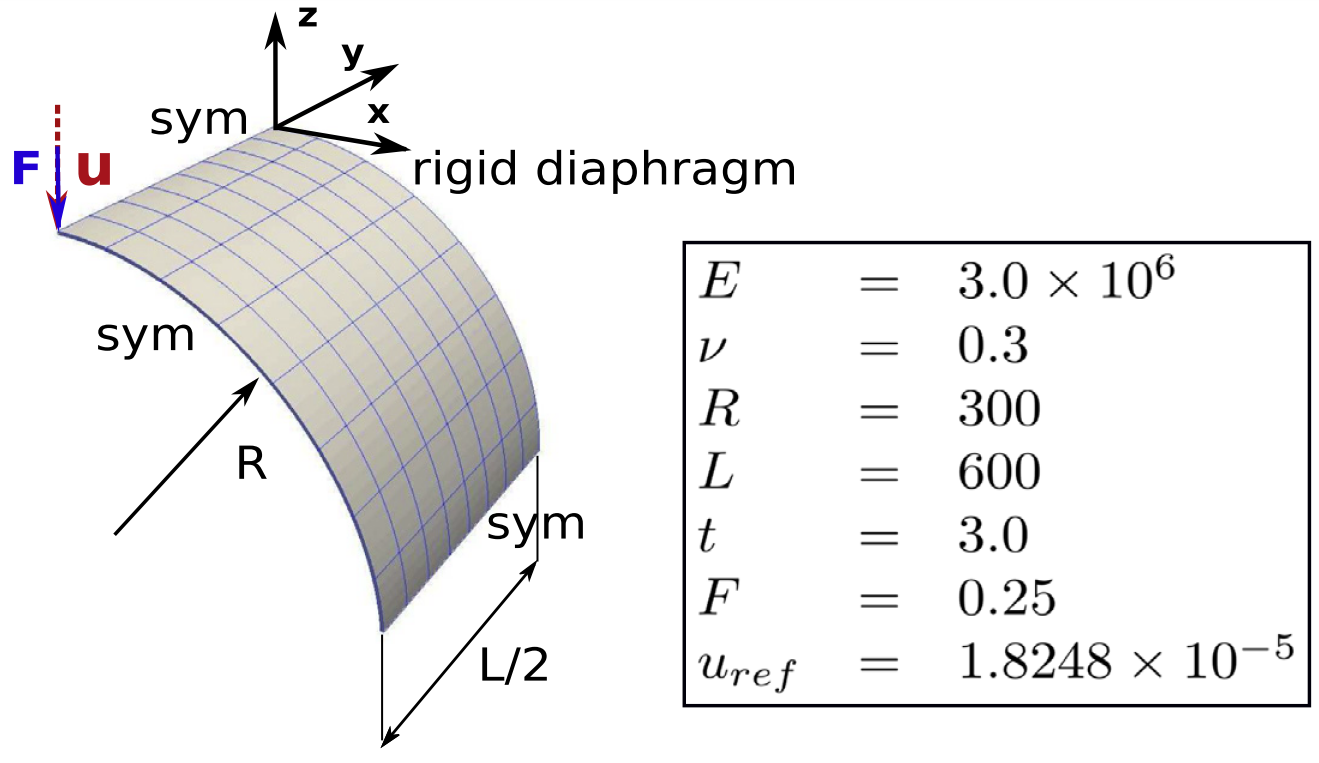
\includegraphics[width=0.4\textwidth]{images/pinchedcylinder.png}
	\caption{Definition of the pinched cylinder benchmark\cite{Bou13}}
\end{wrapfigure}

The pinched cylinder considers a cylindrical shell fixed by rigid diaphragms at it's axial ends. The loading consists of two opposing compressive point loads at the centre of the shell. Due to symmetry only an eighth of the shell is modelled. The key result is the vertical displacement under the point load, denoted by $\textcolor{red}{u}$ in the following diagram. The reference value is $u_{ref} =  1.8248\ \times\ 10^{-5}$. 

 
\begin{figure}[H]
	\subfloat[Quadrilateral element convergence for the pinched cylinder benchmark]
	{\label{ref_label2}
		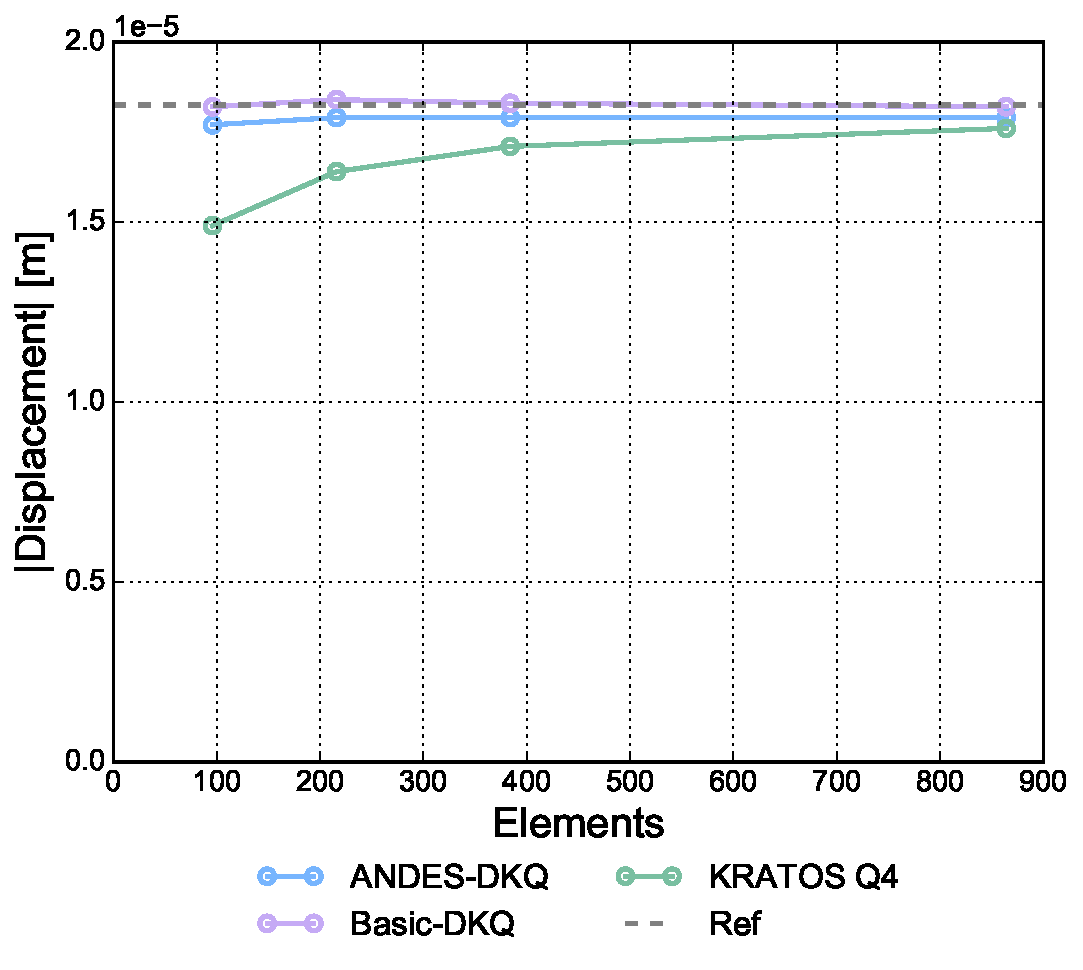
\includegraphics[width=7.3cm]
		{pinched_cyl_structured_quad_results.pdf}}
	\subfloat[Triangle element convergence for the pinched cylinder benchmark]
	{\label{ref_label2}
		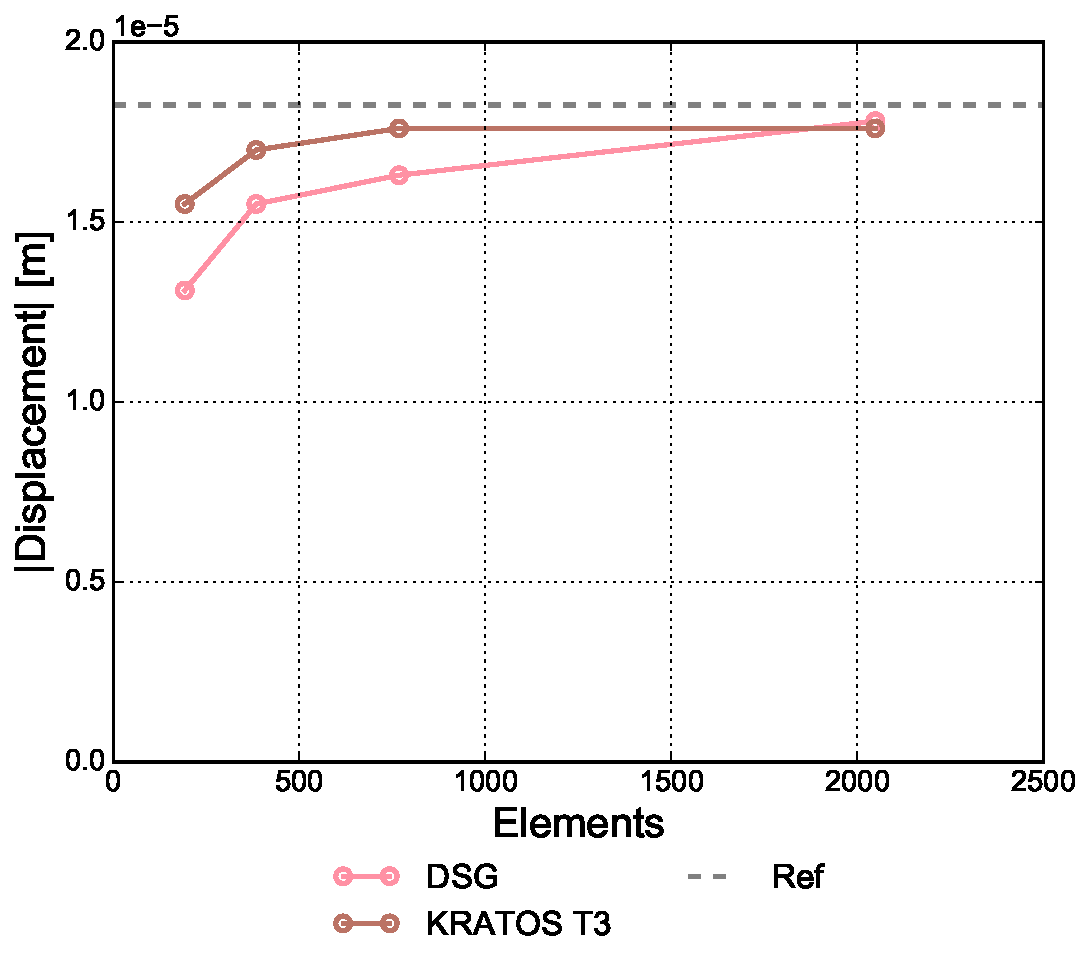
\includegraphics[width=7.3cm]
		{pinched_cyl_structured_tri_results.pdf}}
	\caption{\label{ref_label_overall}Pinched cylinder benchmark results}
\end{figure}

 

Fixup tri results were in the order of 1e-3

The performance of the element is demonstrated in the convergence graph above. It is clear that the element agrees with the reference solution.

\subsection{Pinched hemisphere}

\begin{wrapfigure}{r}{0.45\textwidth}
	\centering
	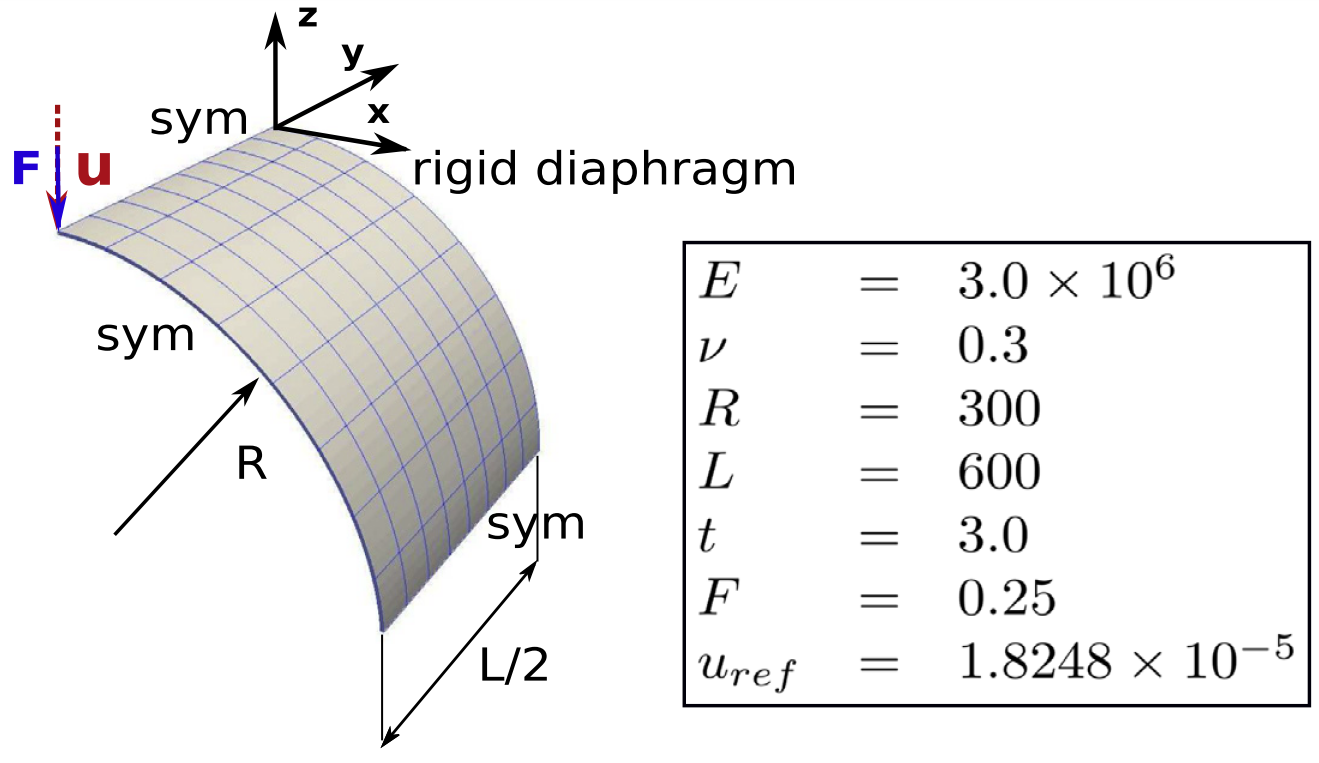
\includegraphics[width=0.4\textwidth]{images/pinchedcylinder.png}
	\caption{Definition of the pinched hemisphere benchmark \cite{Bou13}}
\end{wrapfigure}

The pinched hemisphere considers a hemispherical shell loaded with opposing point loads along it's equator. Due to symmetry only a quarter of the shell is modelled. The key result is the 'x' displacement along one of the point loads, denoted by $\textcolor{red}{u}$ in the following diagram. The reference value is $u_{ref} =  0.0924$. 


\begin{figure}[H]
	\subfloat[Quadrilateral element convergence for the pinched hemisphere benchmark]
	{\label{ref_label2}
		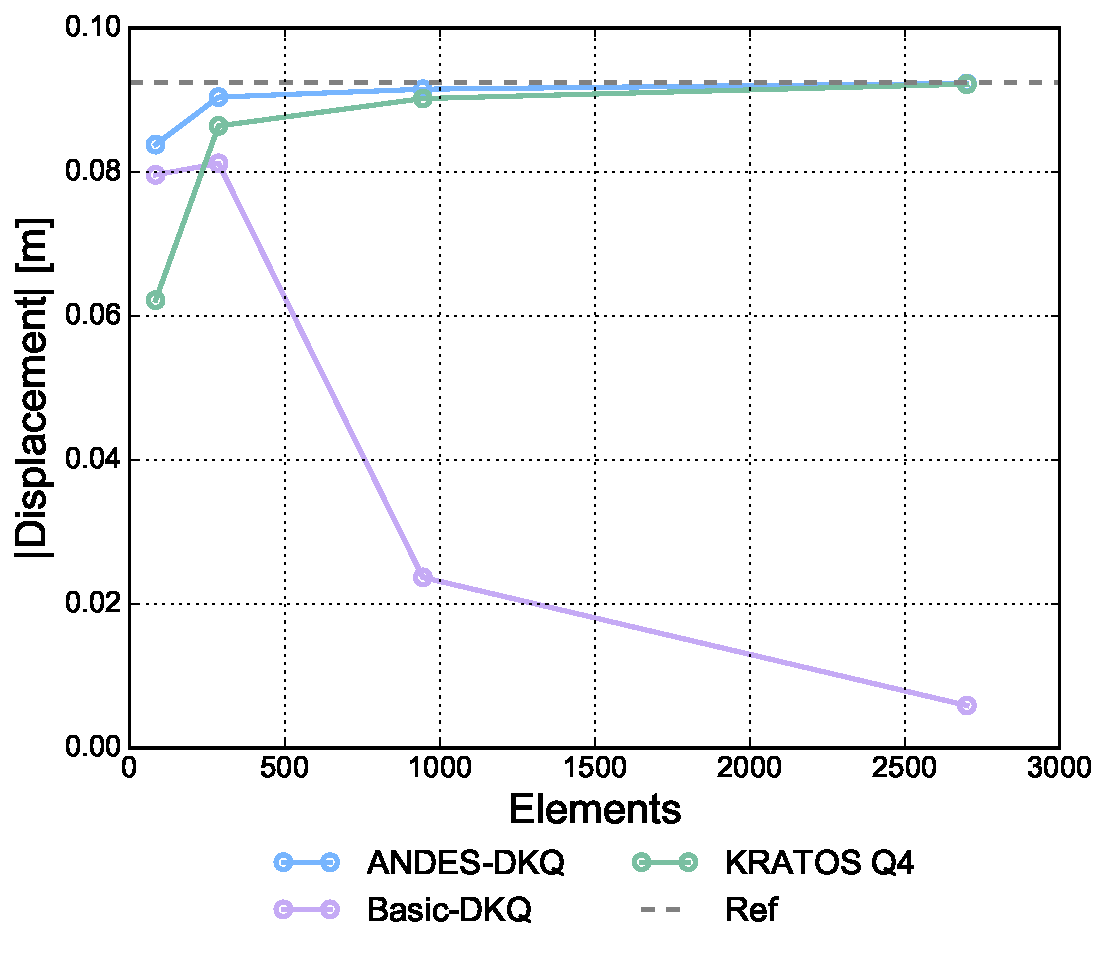
\includegraphics[width=7.3cm]
		{pinched_hemi_quad_results.pdf}}
	\subfloat[Triangle element convergence for the pinched hemisphere benchmark]
	{\label{ref_label2}
		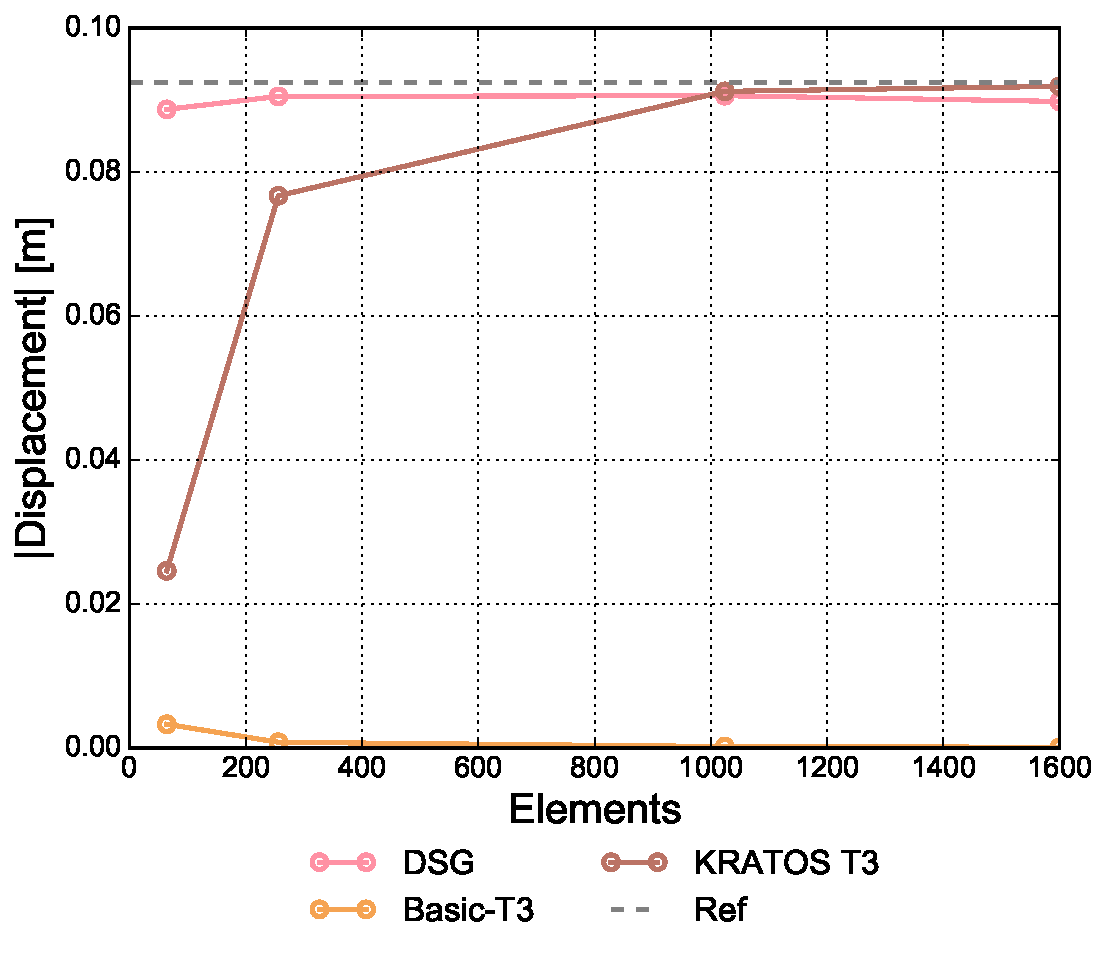
\includegraphics[width=7.3cm]
		{pinched_hemi_tri_results.pdf}}
	\caption{\label{ref_label_overall}Pinched hemisphere benchmark results}
\end{figure}

Fixup tri results

Contrary to the previous benchmarks, the element does not converge to the reference solution in the pinched hemisphere test.  A key point to note is that the other benchmarks in the shell obstacle course employ a structured mesh, while the geometry of this test requires an unstructured mesh. Subsequent investigations of the element attempting to isolate remaining formulation issues have revealed the following phenomena:

\section{Geometically nonlinear benchmarks}

asdfasdf

\subsection{Hinged cylindrical roof}

Tests snapthrough

 
\begin{figure}[H]
	%\centering
	\subfloat[Hinged cylindrical roof definition \cite{Sze2004}]
	{\label{ref_label1}
		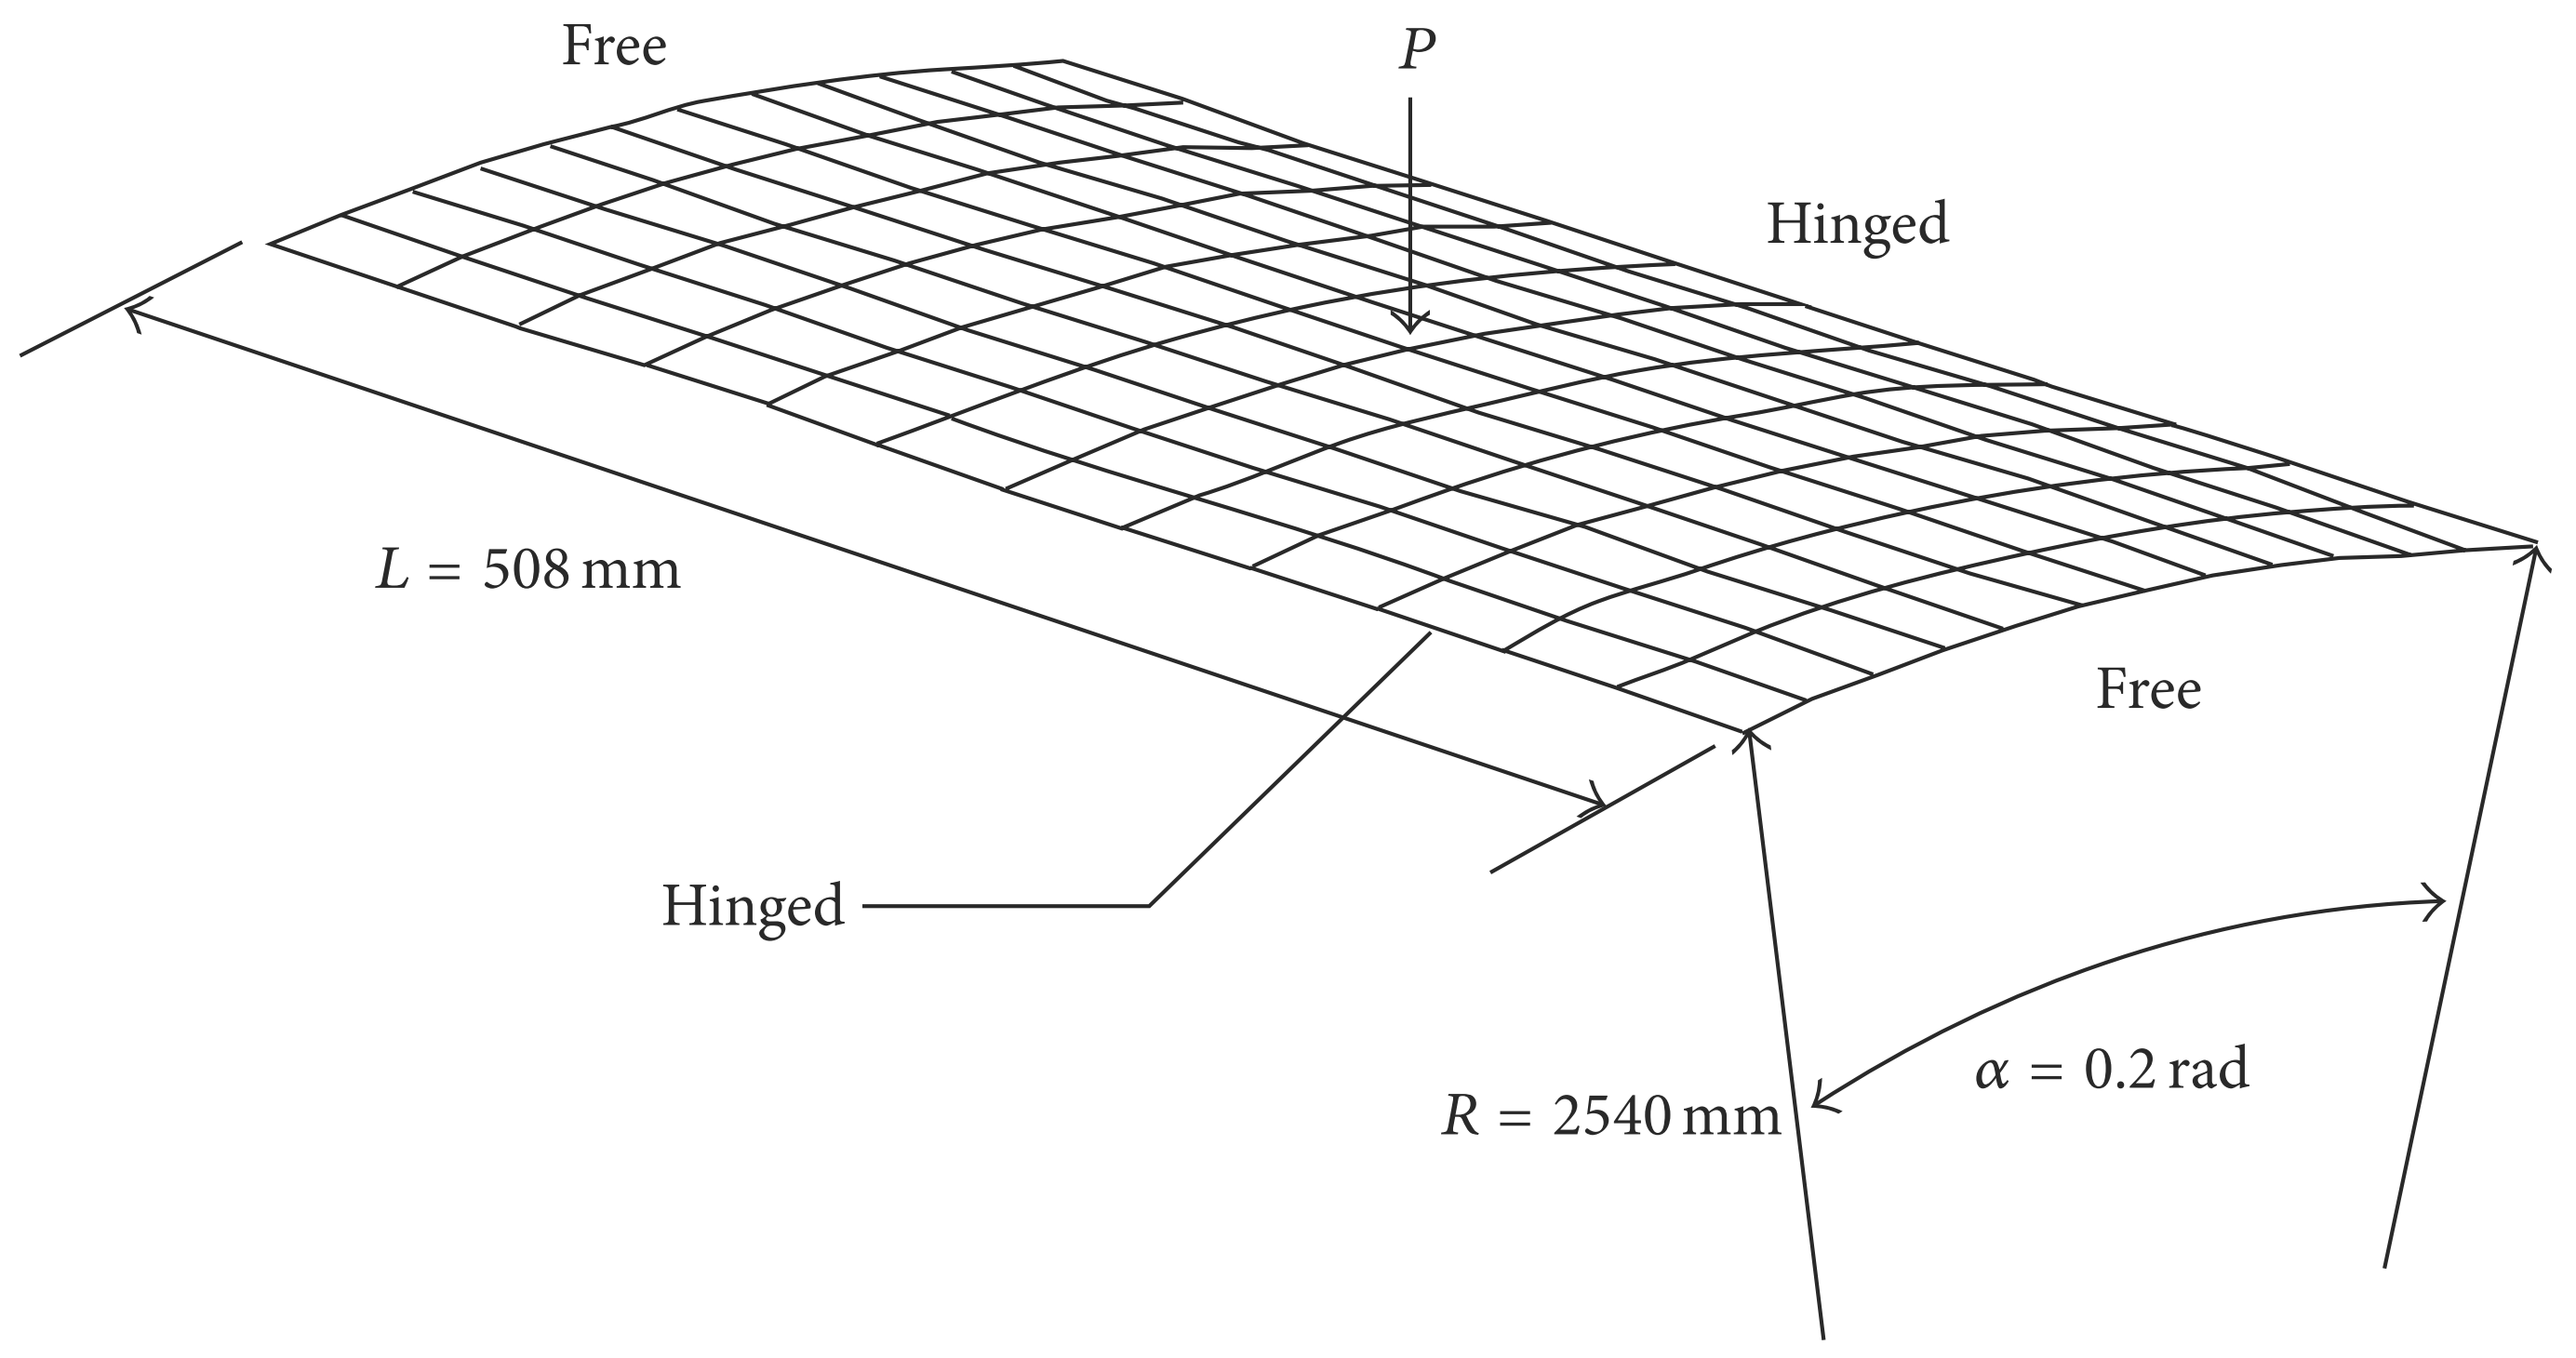
\includegraphics[width=7.3cm]
		{images/hinged_cylindrical_roof.png}}
	\subfloat[Load-displacement curve of hinged cylindrical roof]
	{\label{ref_label2}
		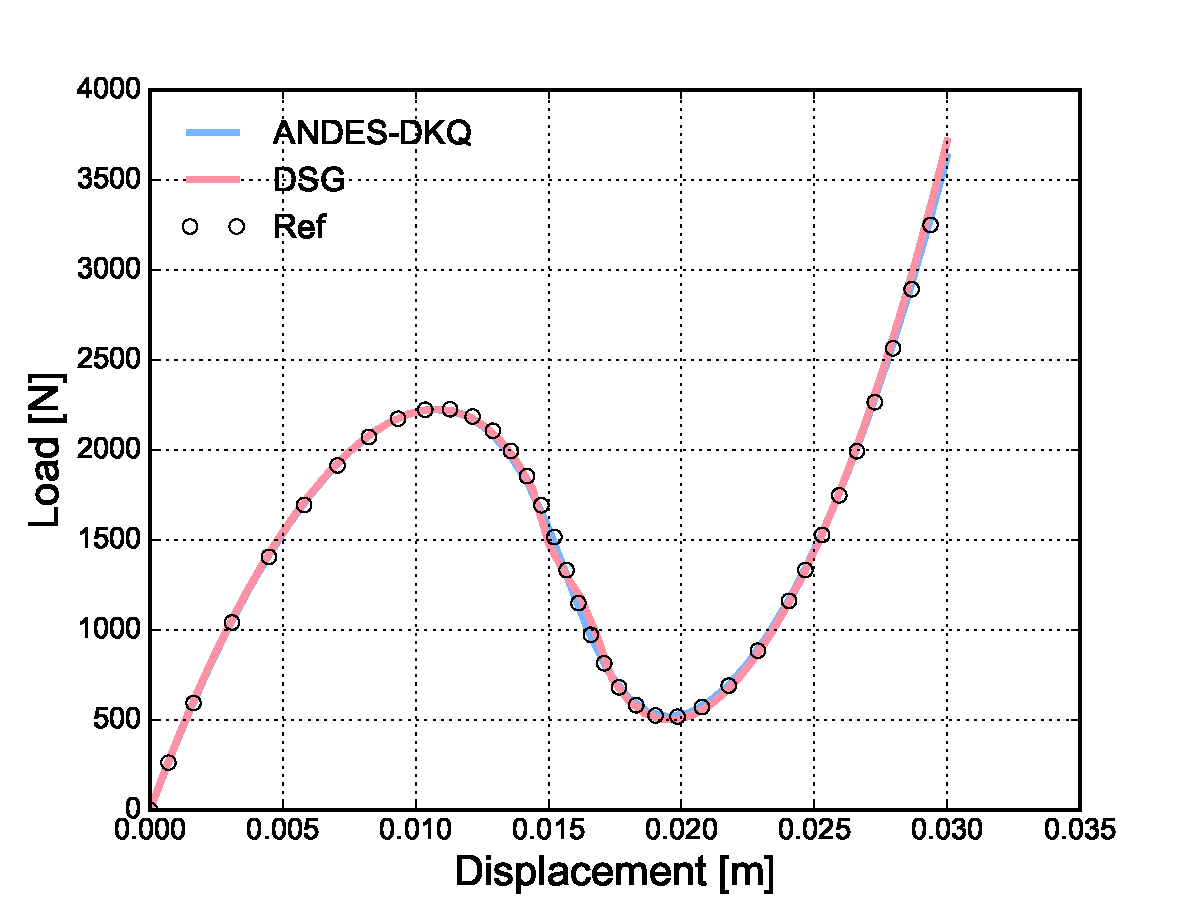
\includegraphics[width=7.3cm]
		{Load_displacement_curve_hinged_cylindrical_roof.pdf}}
	\caption{\label{ref_label_overall}Hinged cylindrical roof benchmark}
\end{figure}

 

reference solution from \cite{Sze2004}

\subsection{Open cylinder pullout}

pullout problem

 
\begin{figure}[H]
	%\centering
	\subfloat[Open cylinder pullout definition \cite{Sze2004}]
	{\label{ref_label1}
		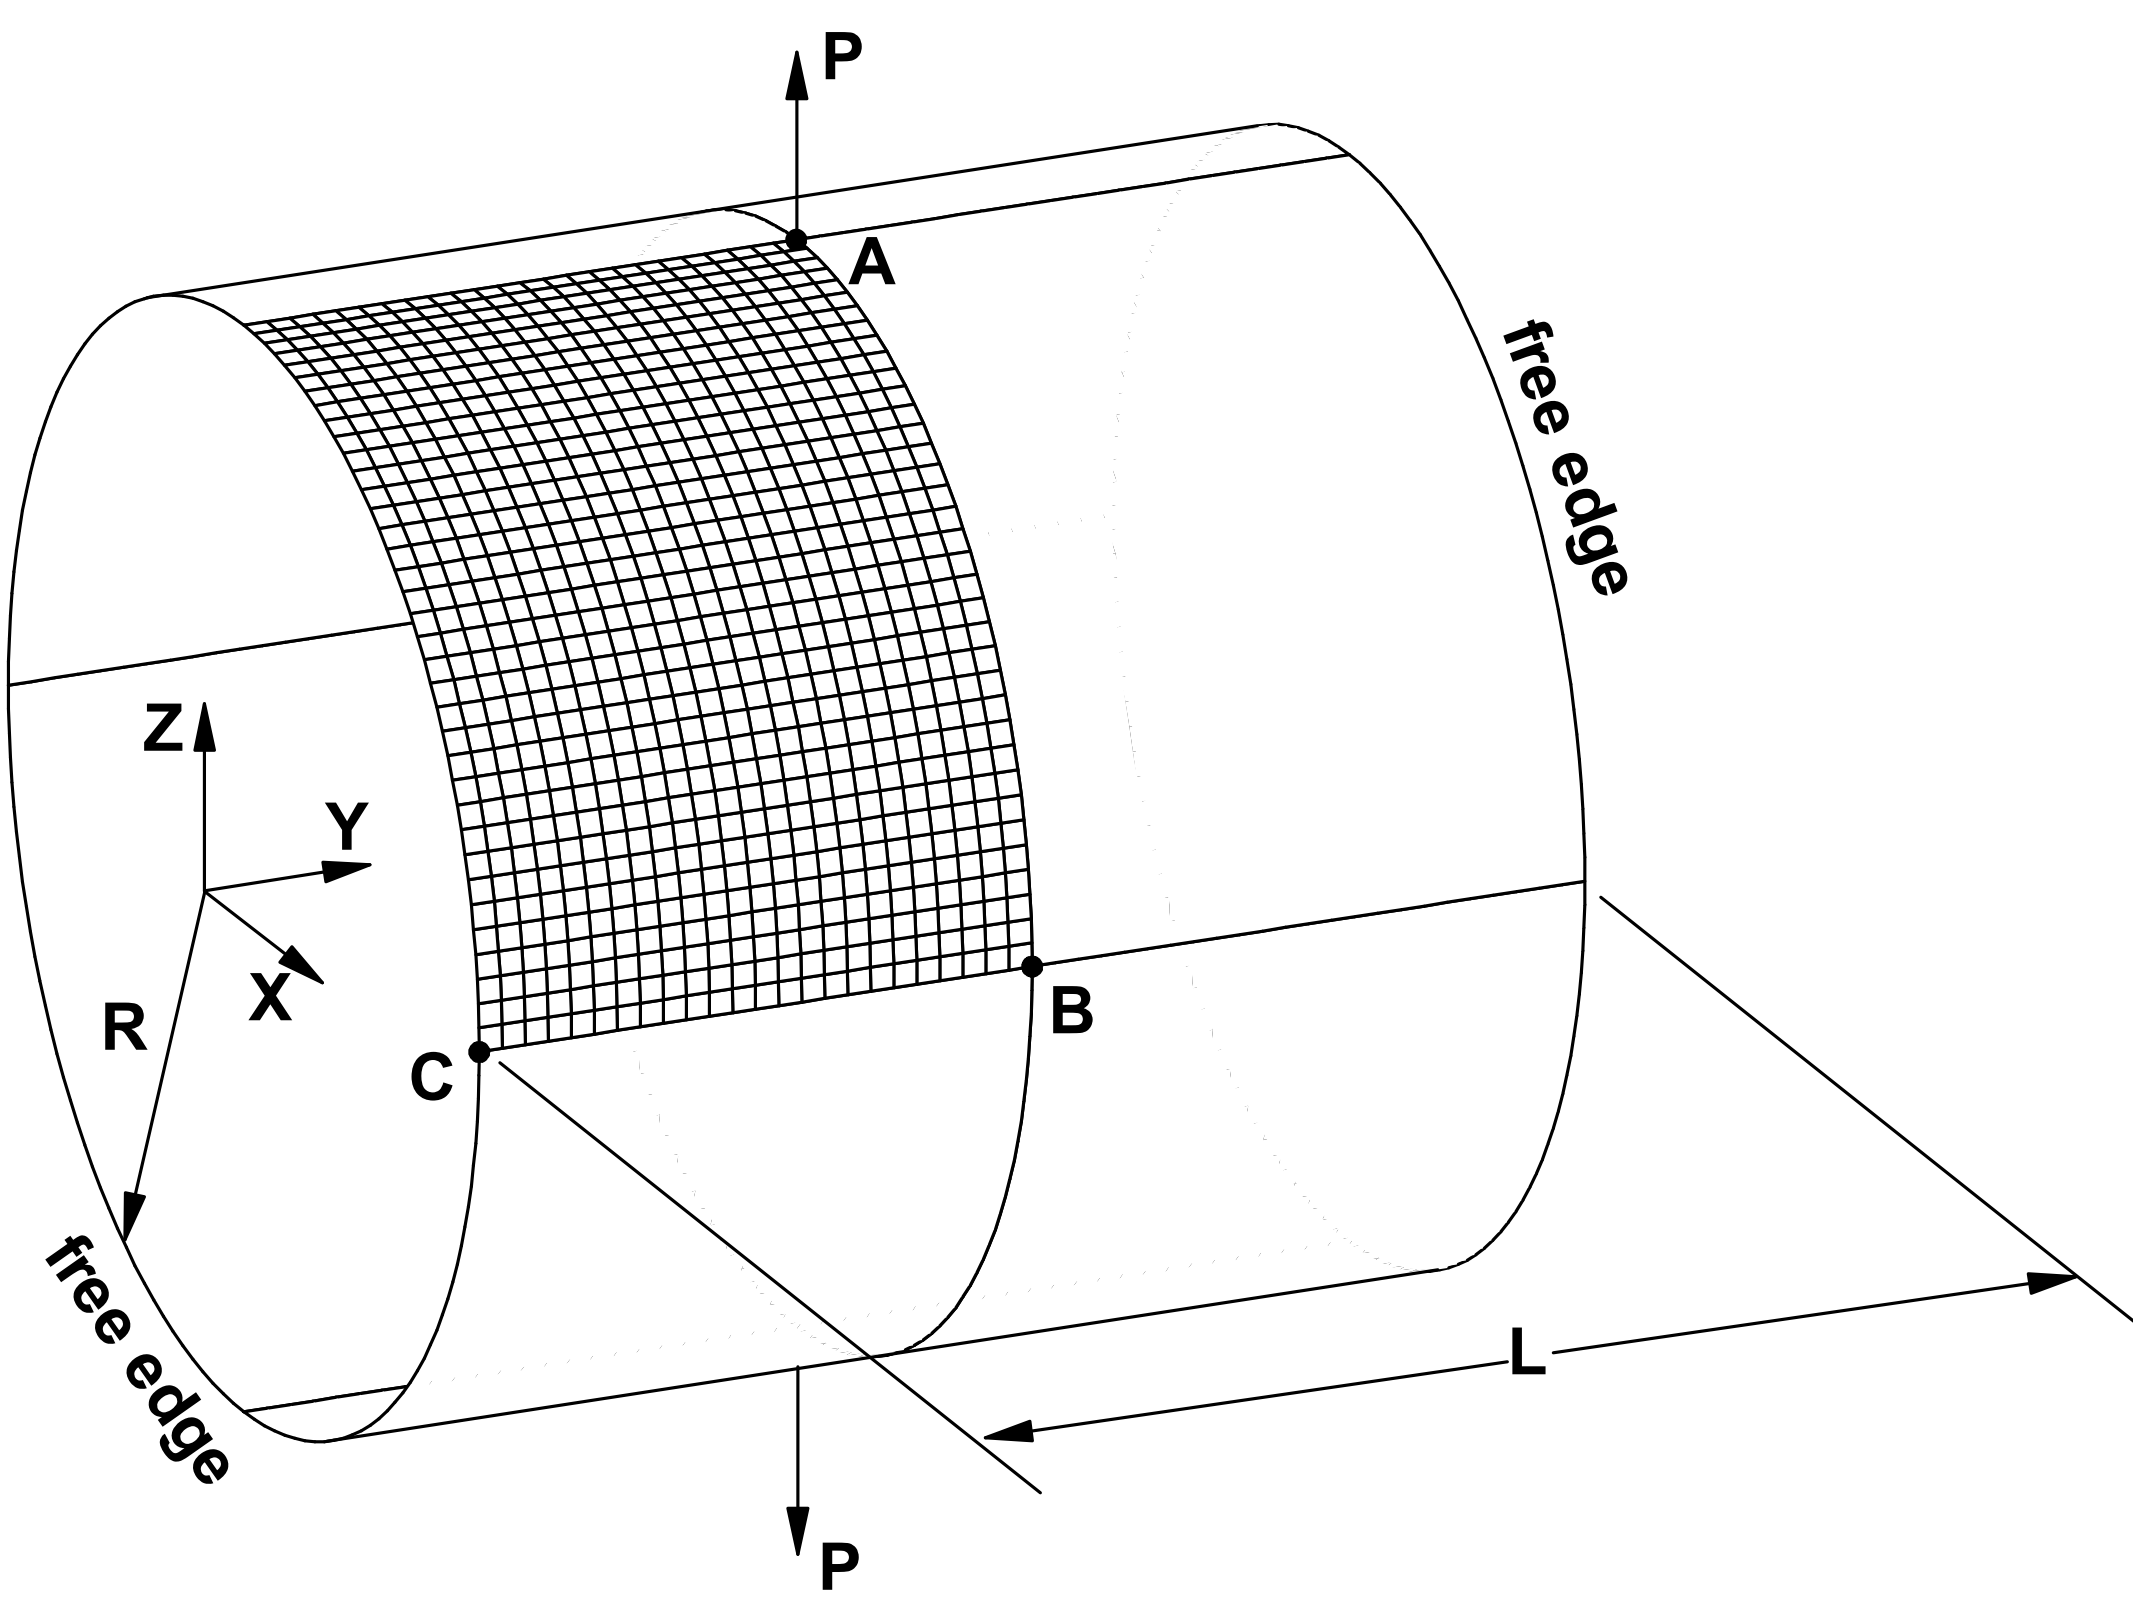
\includegraphics[width=7.3cm]
		{images/opencylinderpullout.png}}
	\subfloat[Load-displacement curve of open cylinder pullout]
	{\label{ref_label2}
		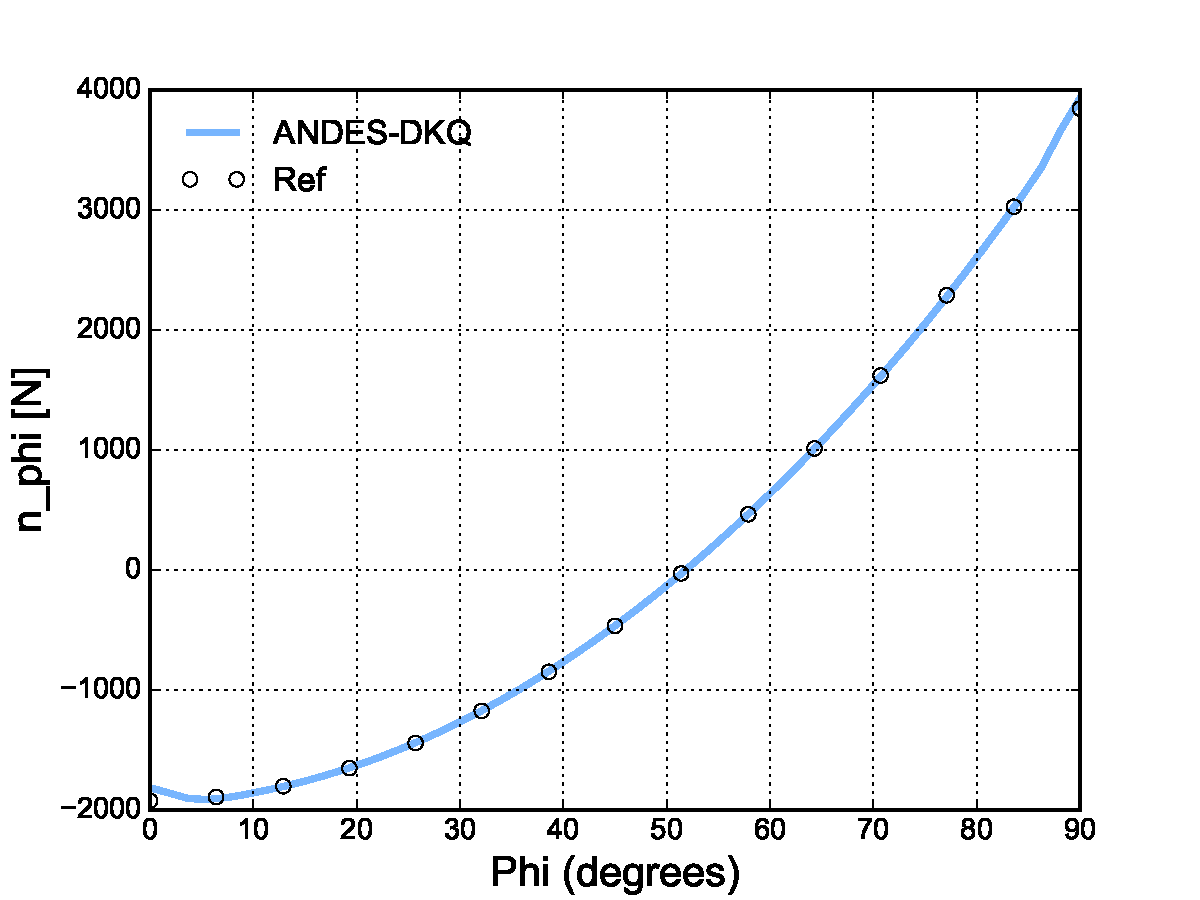
\includegraphics[width=7.3cm]
		{Load_displacement_curve_open_cylinder_pullout.pdf}}
	\caption{\label{ref_label_overall}Open cylinder pullout benchmark}
\end{figure}

 

asdfasdf

\section{Dynamics benchmarks}

asdfasdf

\subsection{Shell pendulum}

asdfasdf

 
\begin{figure}[H]
	%\centering
	\subfloat[Shell pendulum definition]
	{\label{ref_label1}
		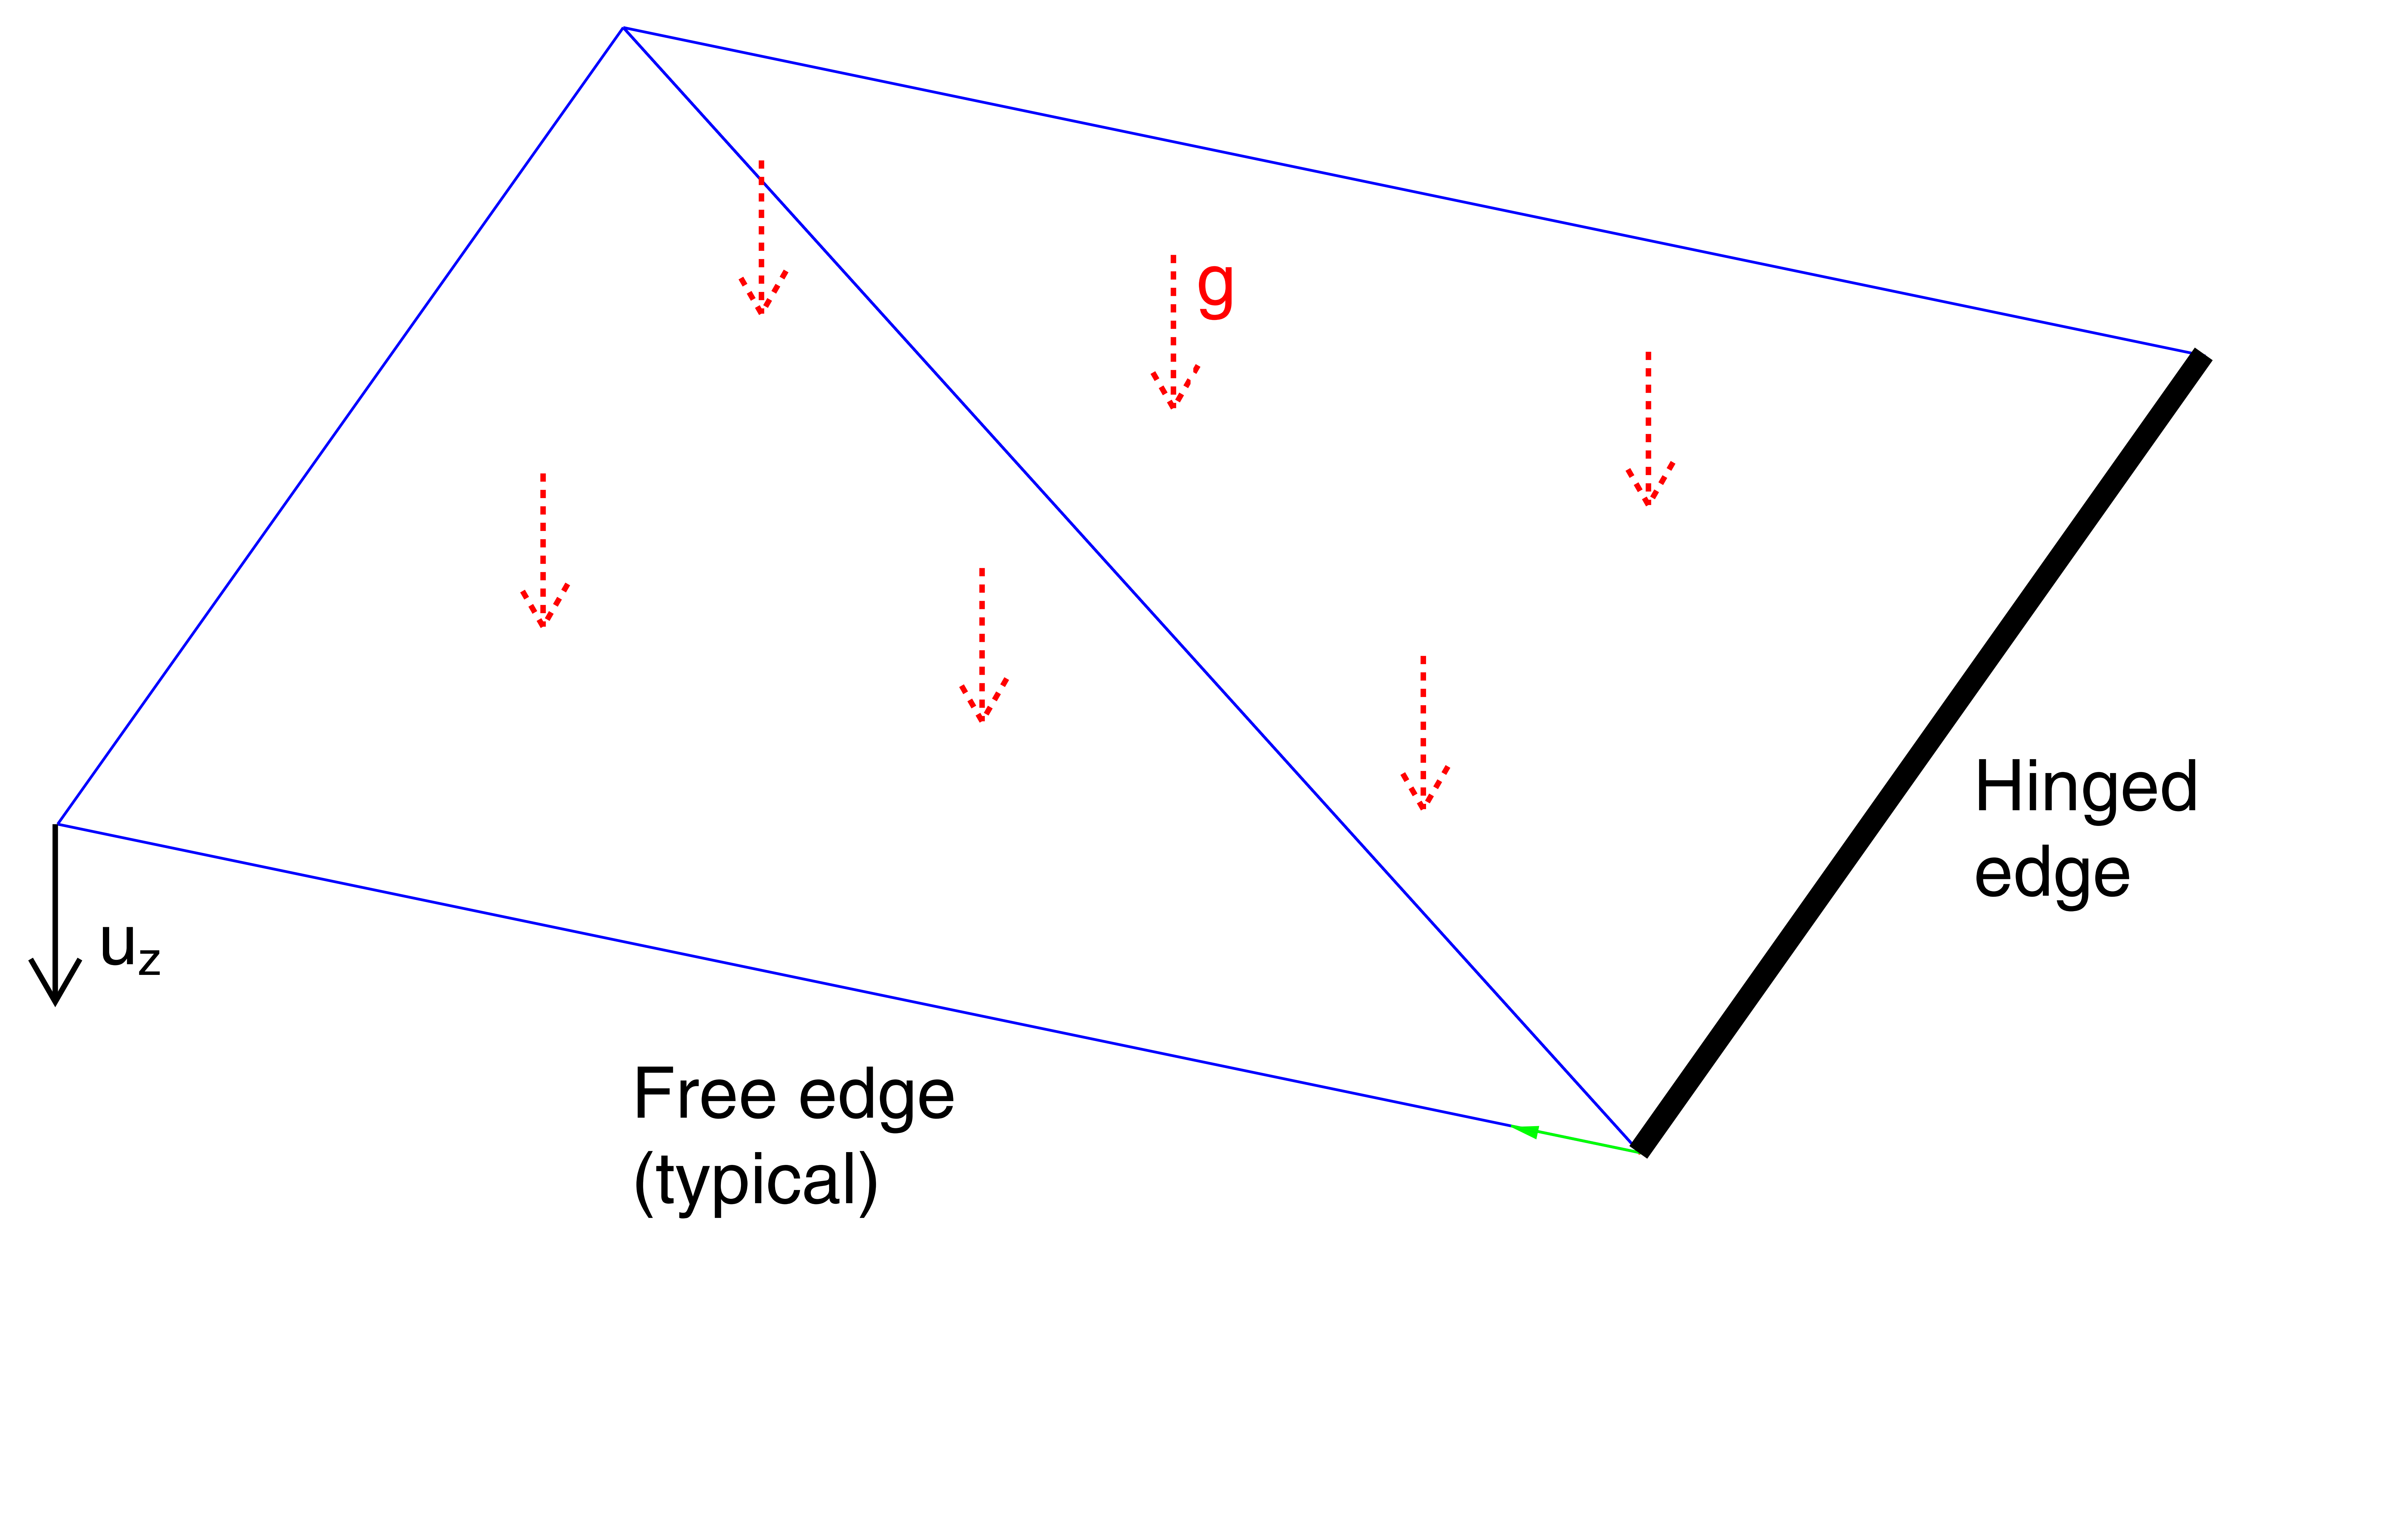
\includegraphics[width=7.3cm]
		{images/swinging_plate_problem.png}}
	\subfloat[Vertical displacement over time for shell pendulum benchmark]
	{\label{ref_label2}
		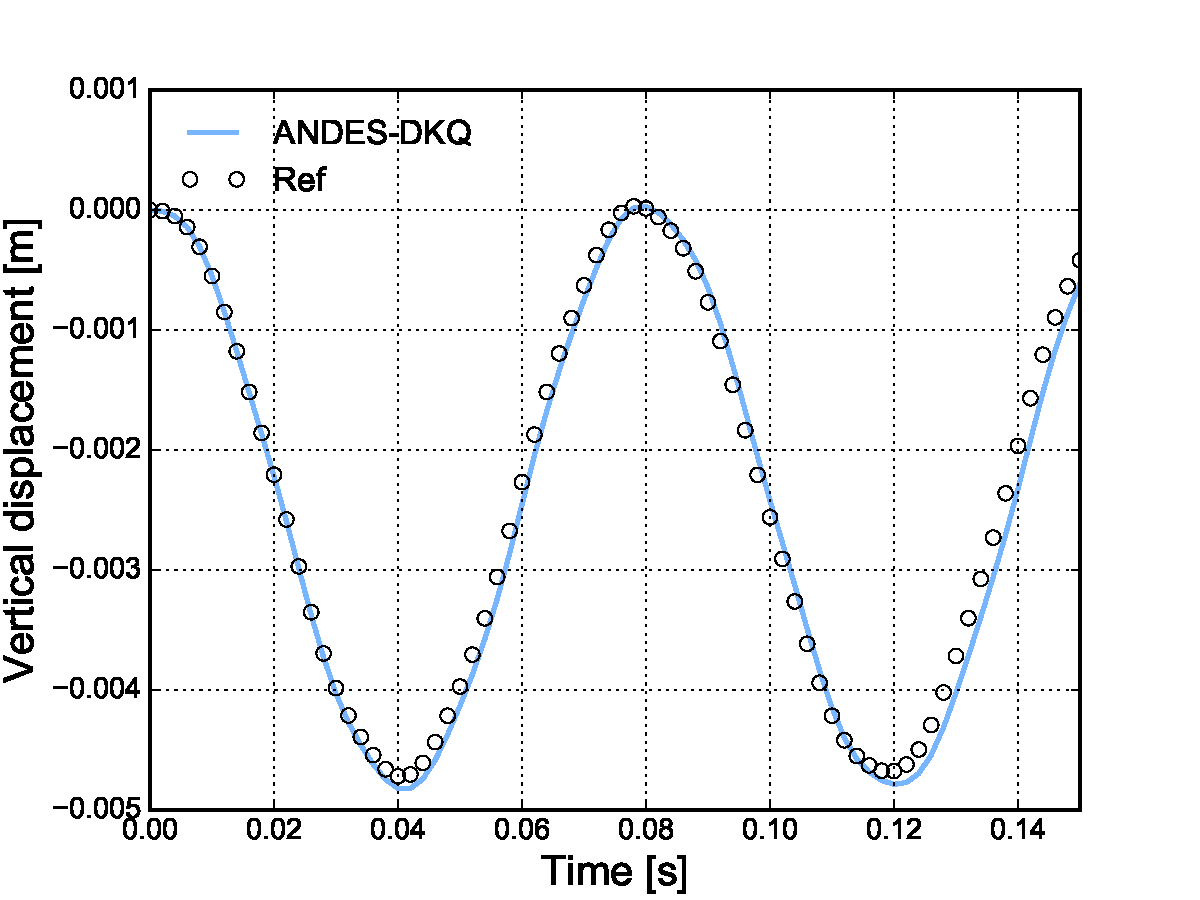
\includegraphics[width=7.3cm]
		{swinging_plate_graph.pdf}}
	\caption{\label{ref_label_overall}Shell pendulum benchmark}
\end{figure}

 

ref is existing kratos quad

asfsdf

\subsection{Oscillating clamped plate}

adfdas


 
\begin{figure}[H]
	%\centering
	\subfloat[Oscillating clamped plate definition]
	{\label{ref_label1}
		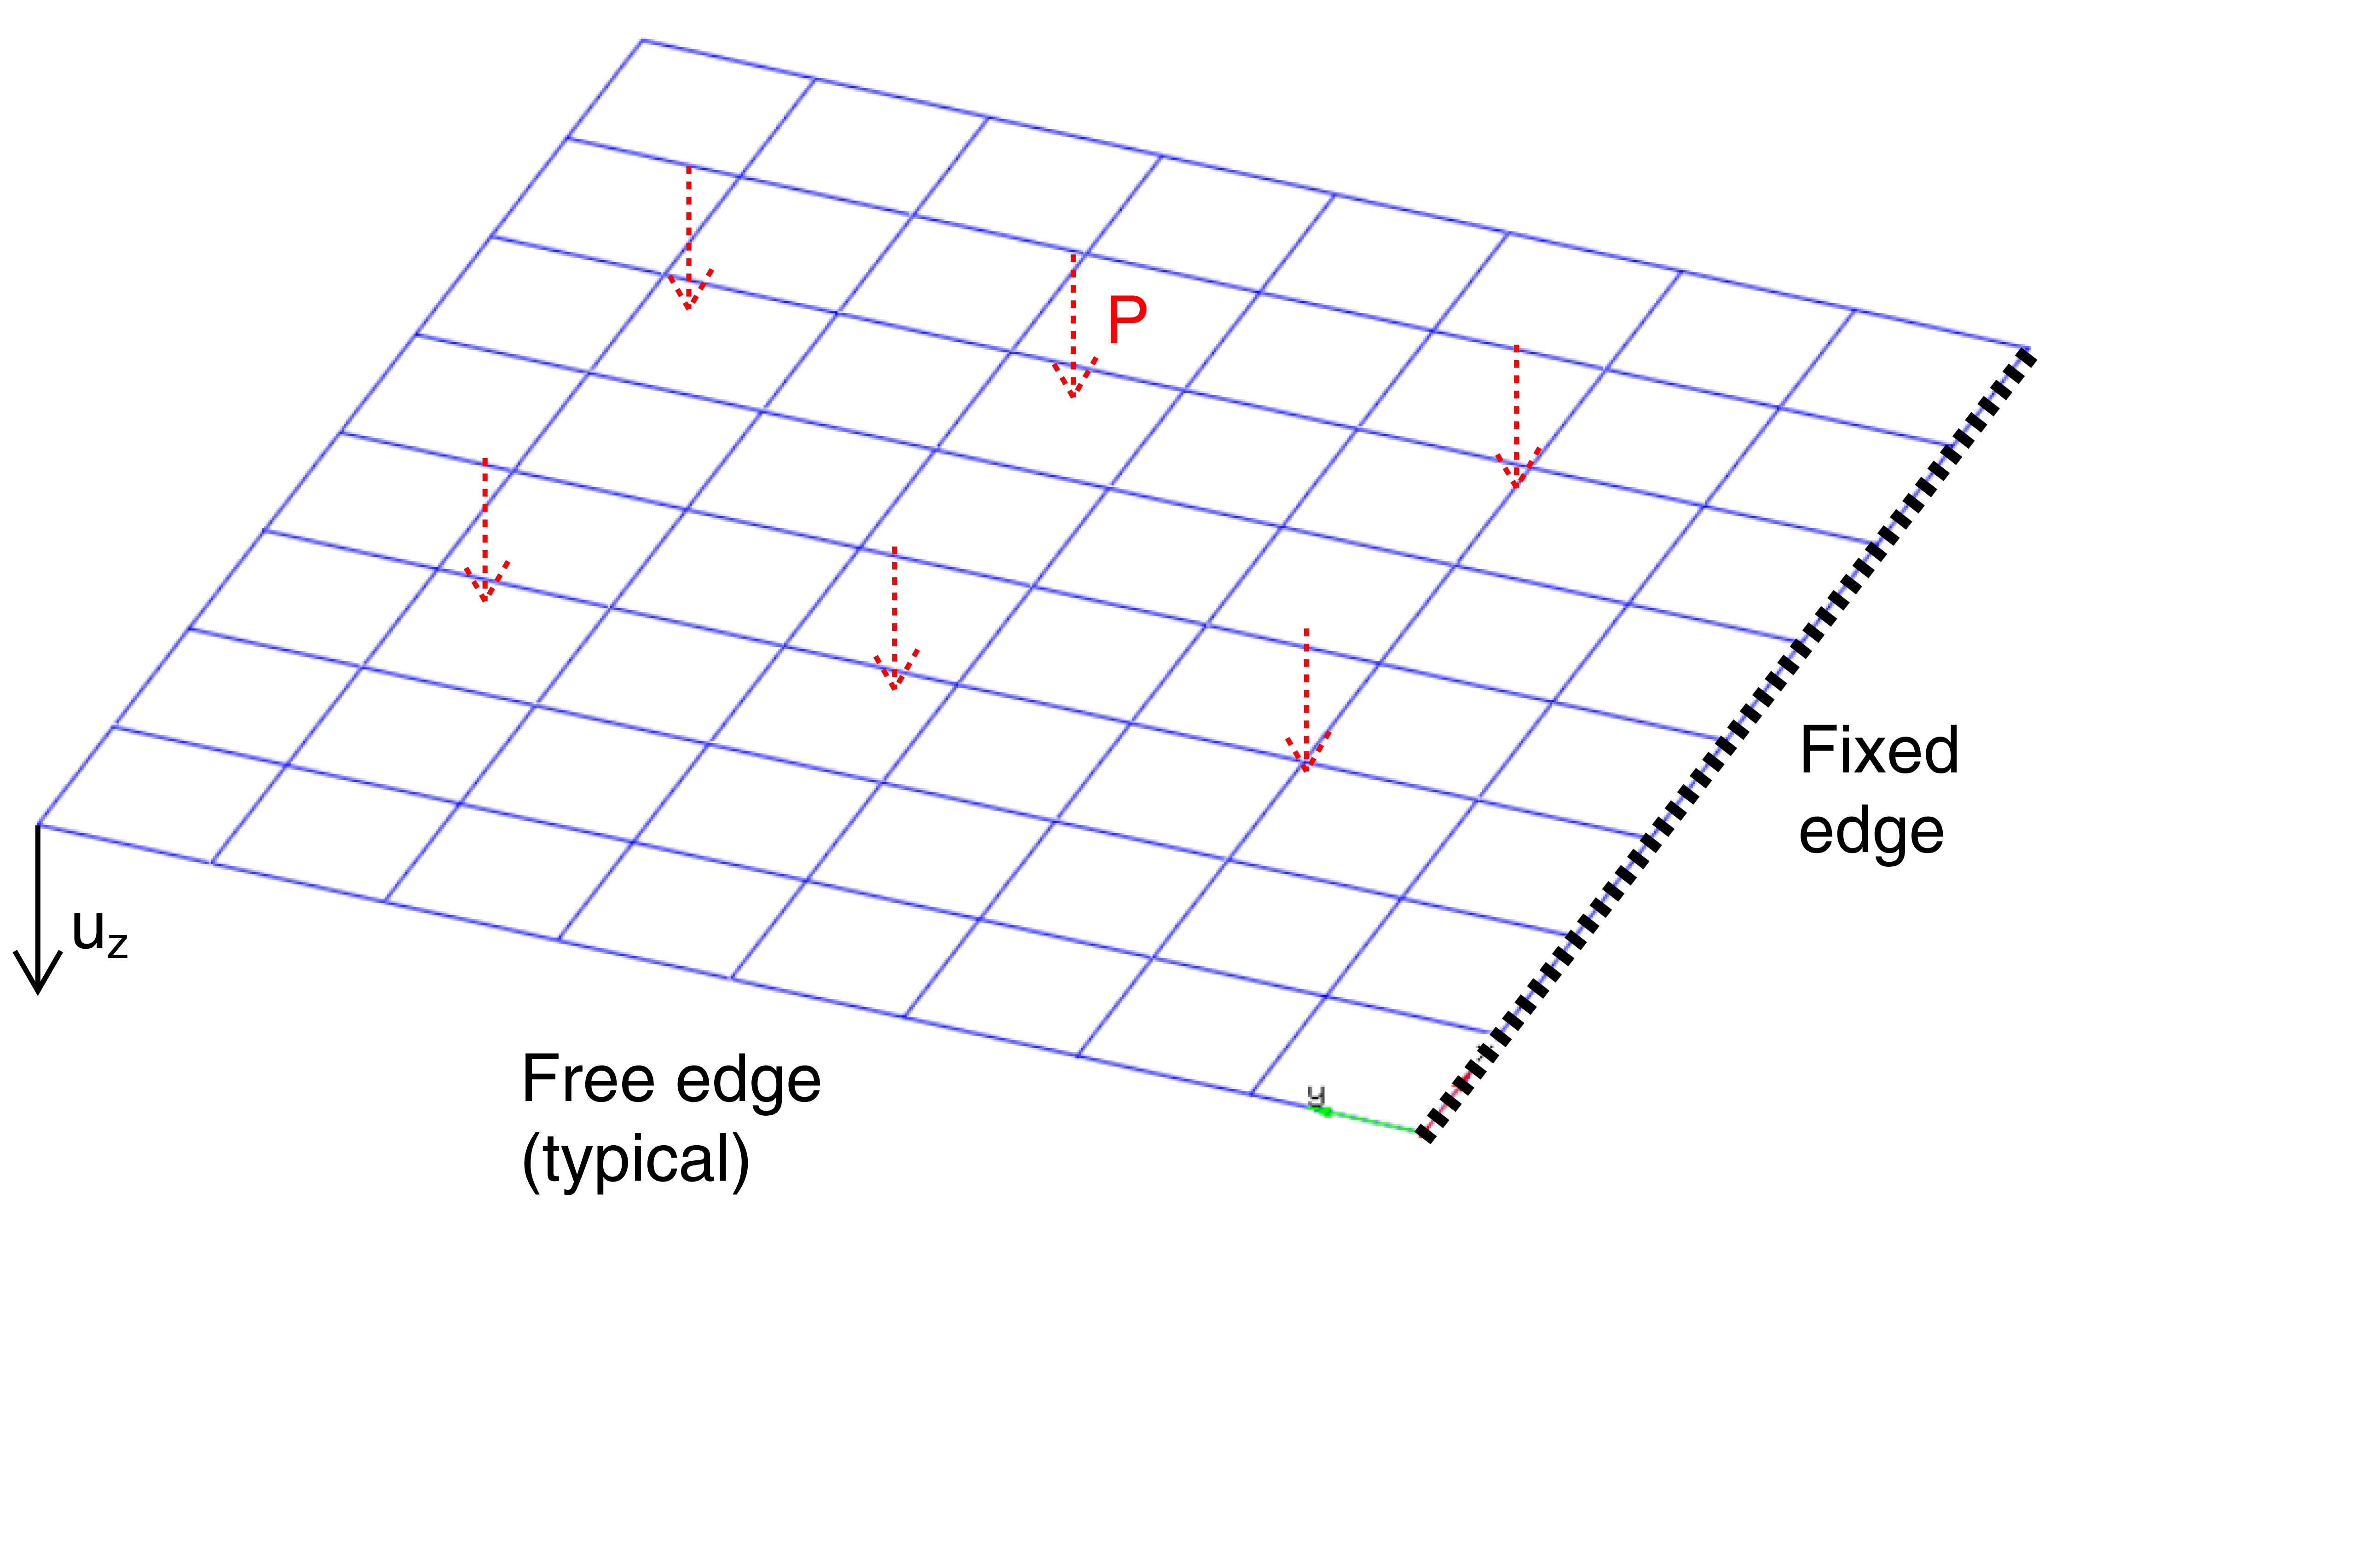
\includegraphics[width=7.3cm]
		{images/quad_bend_problem.png}}
	\subfloat[Vertical displacement over time for Oscillating clamped plate benchmark]
	{\label{ref_label2}
		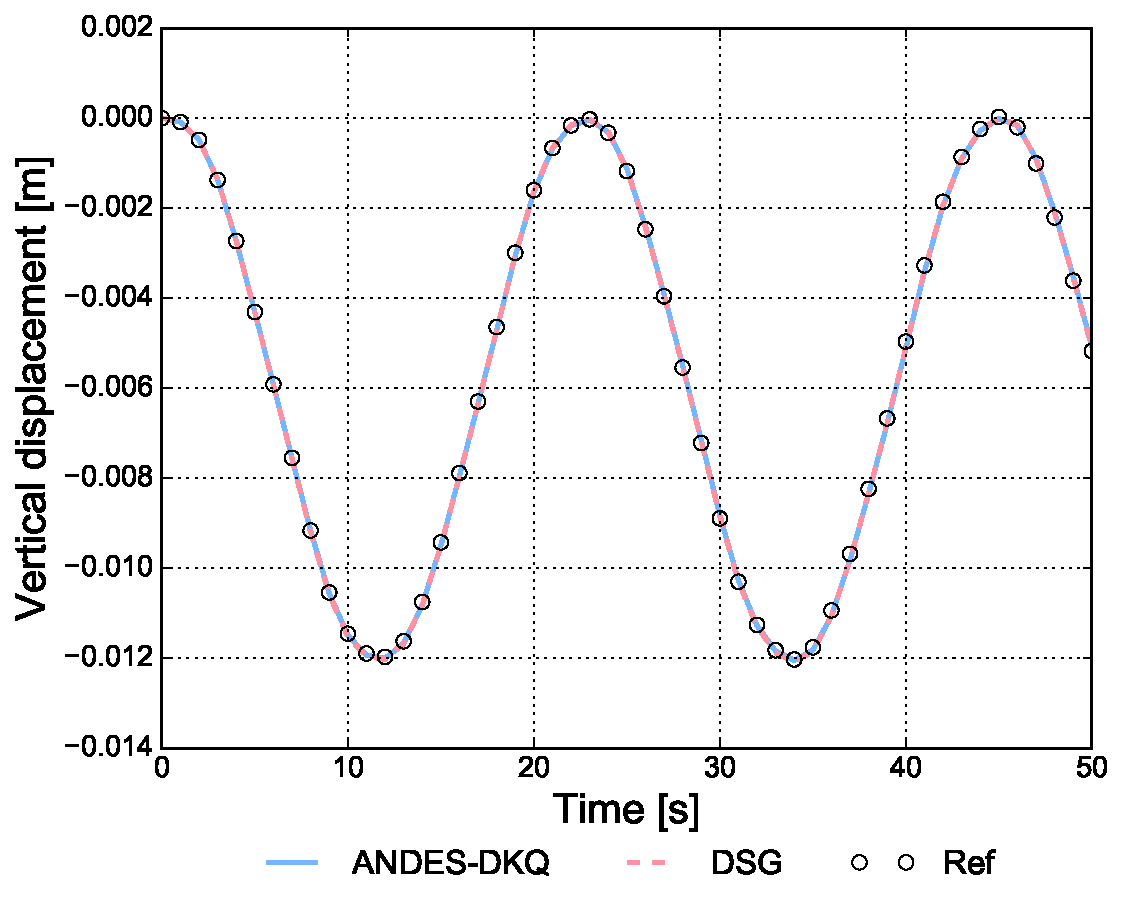
\includegraphics[width=7.3cm]
		{quad_bend_graph.pdf}}
	\caption{\label{Oscillating clamped plate benchmark}Oscillating clamped plate benchmark}
\end{figure}

 

ref is existing kratos quad

\section{Quantity recovery benchmarks}

asdfasdf



\subsection{Snow loaded dome}

ToS-cyk-Assignment09.pdf

\subsection{LEFM SIF recovery}

poisson != 0
check strains, forces, moments

\begin{figure}[H]
	%\centering
	\subfloat[LEFM stress concentration factor recovery definition]
	{\label{ref_label1}
		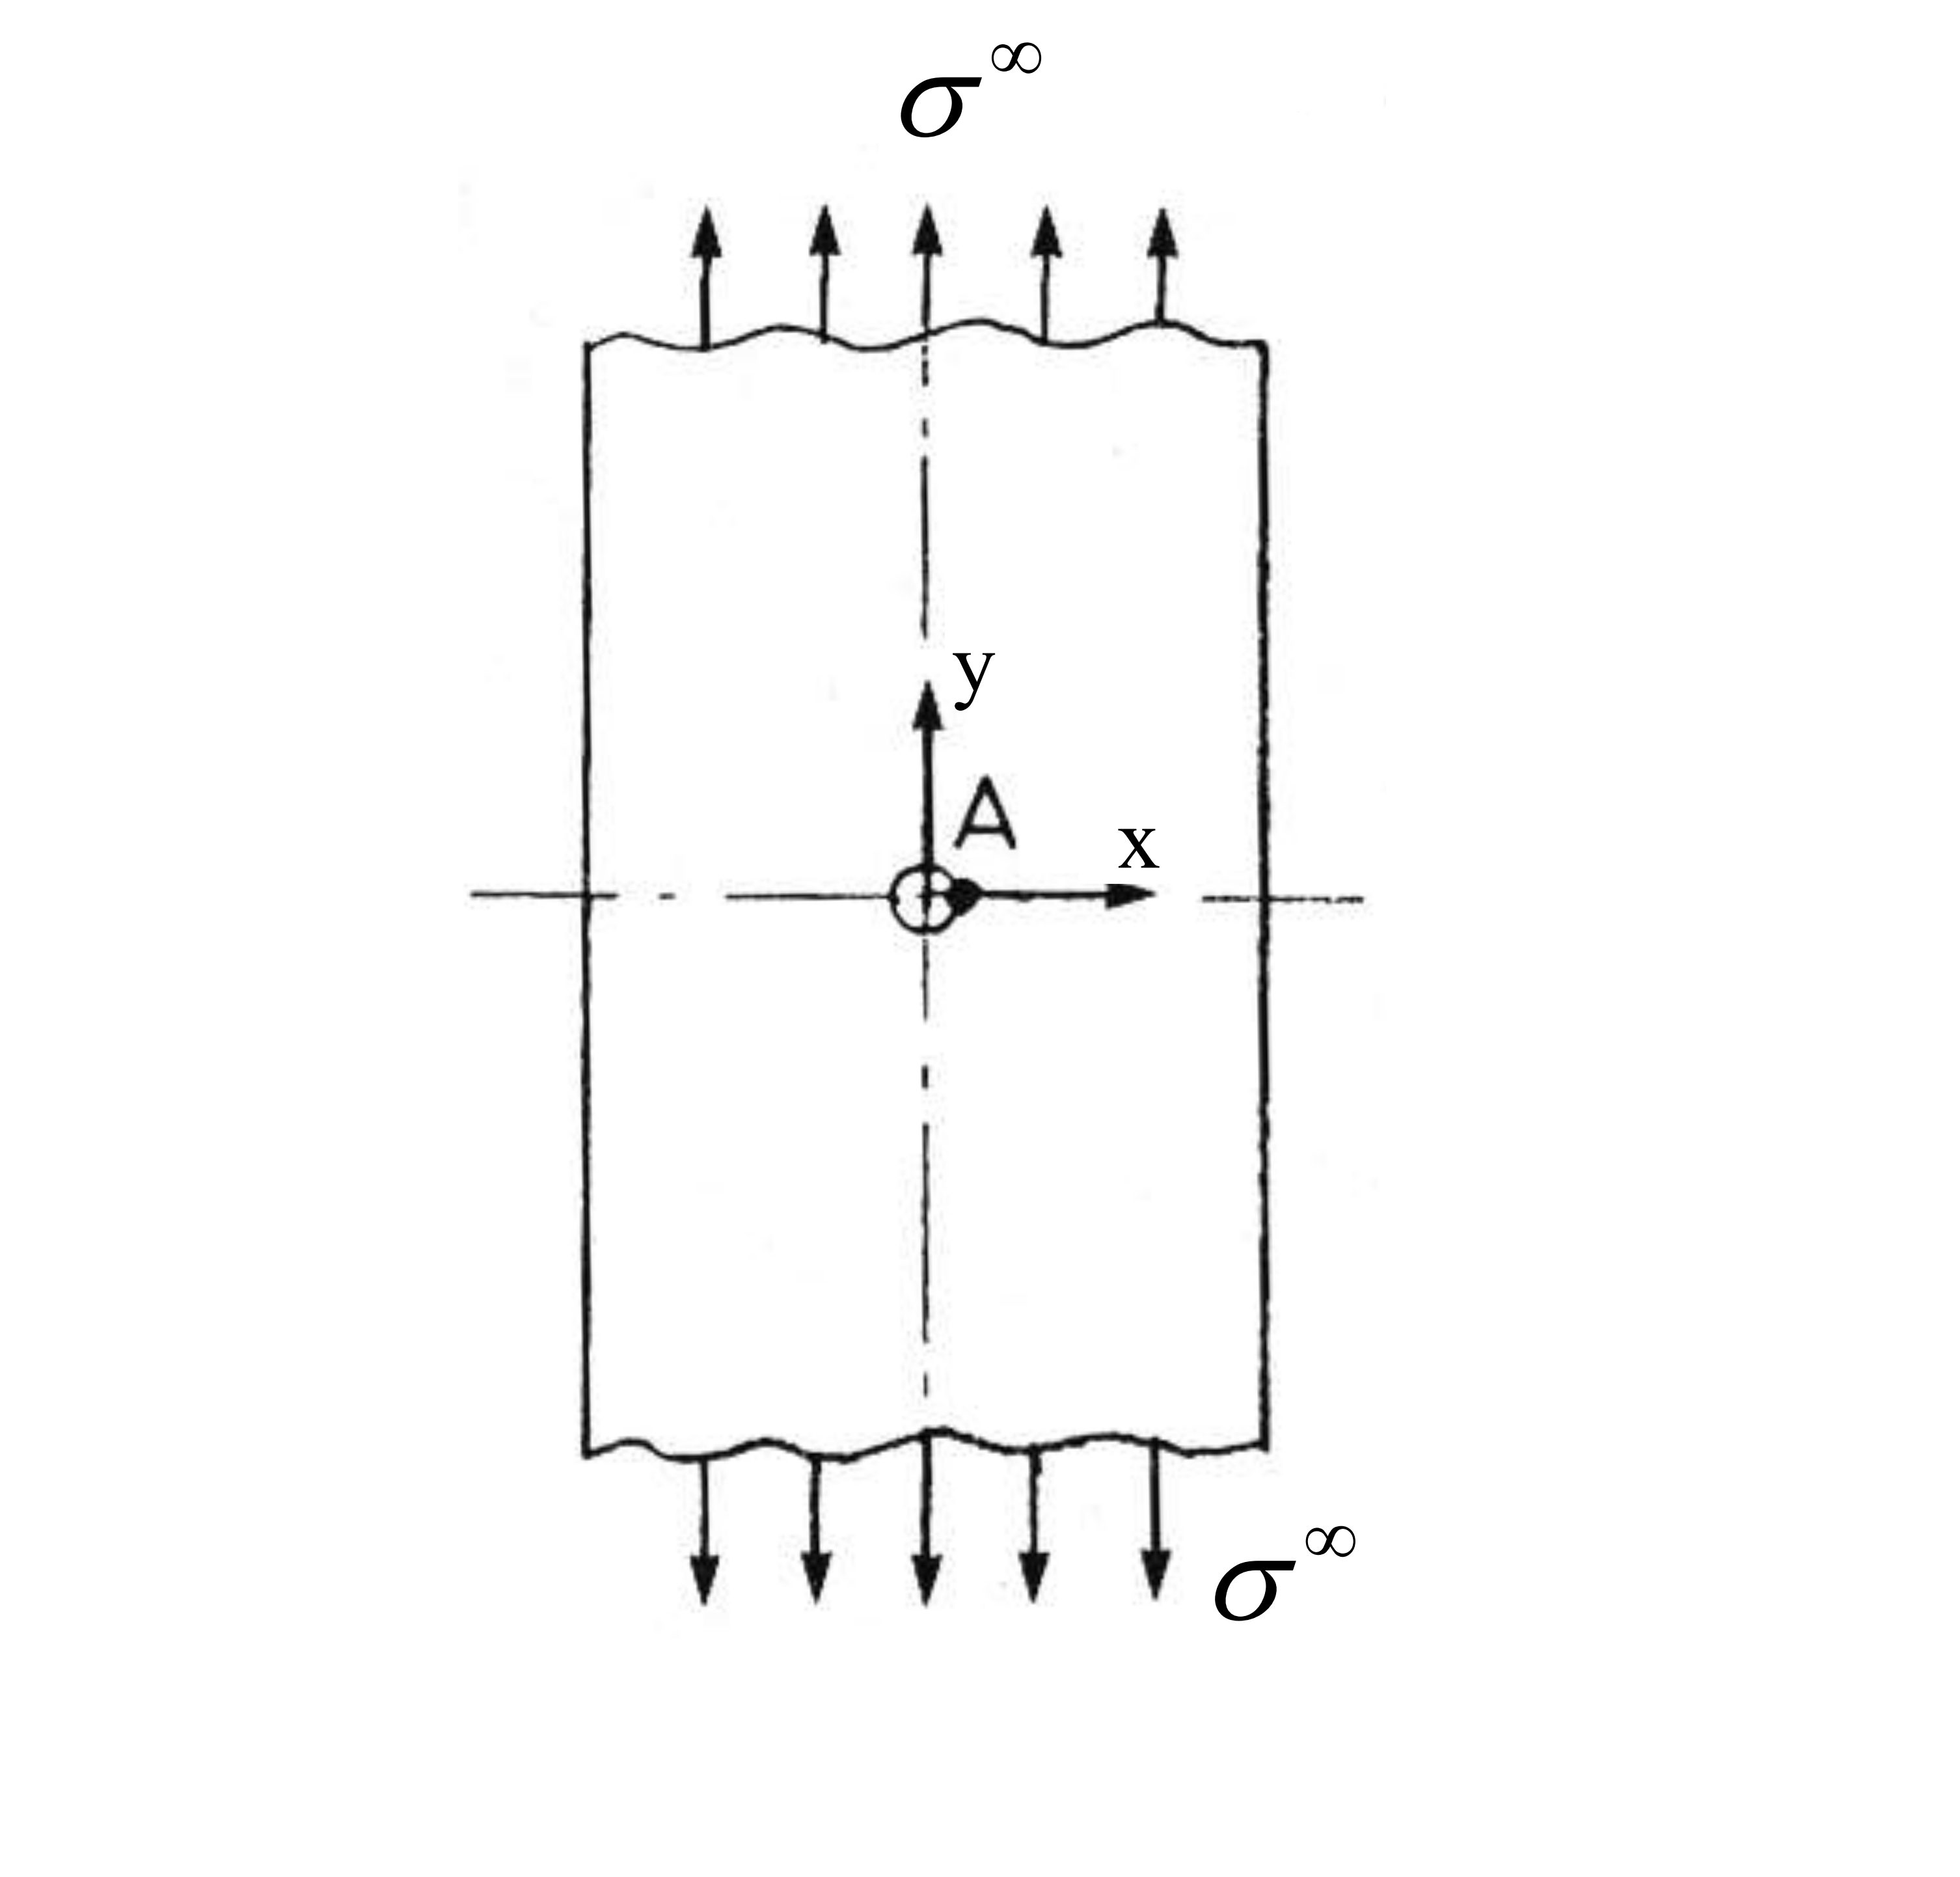
\includegraphics[width=7.3cm]
		{images/plate_with_hole_definition.png}}
	\subfloat[Stress distribution along distance from hole for LEFM stress concentration factor benchmark]
	{\label{ref_label2}
		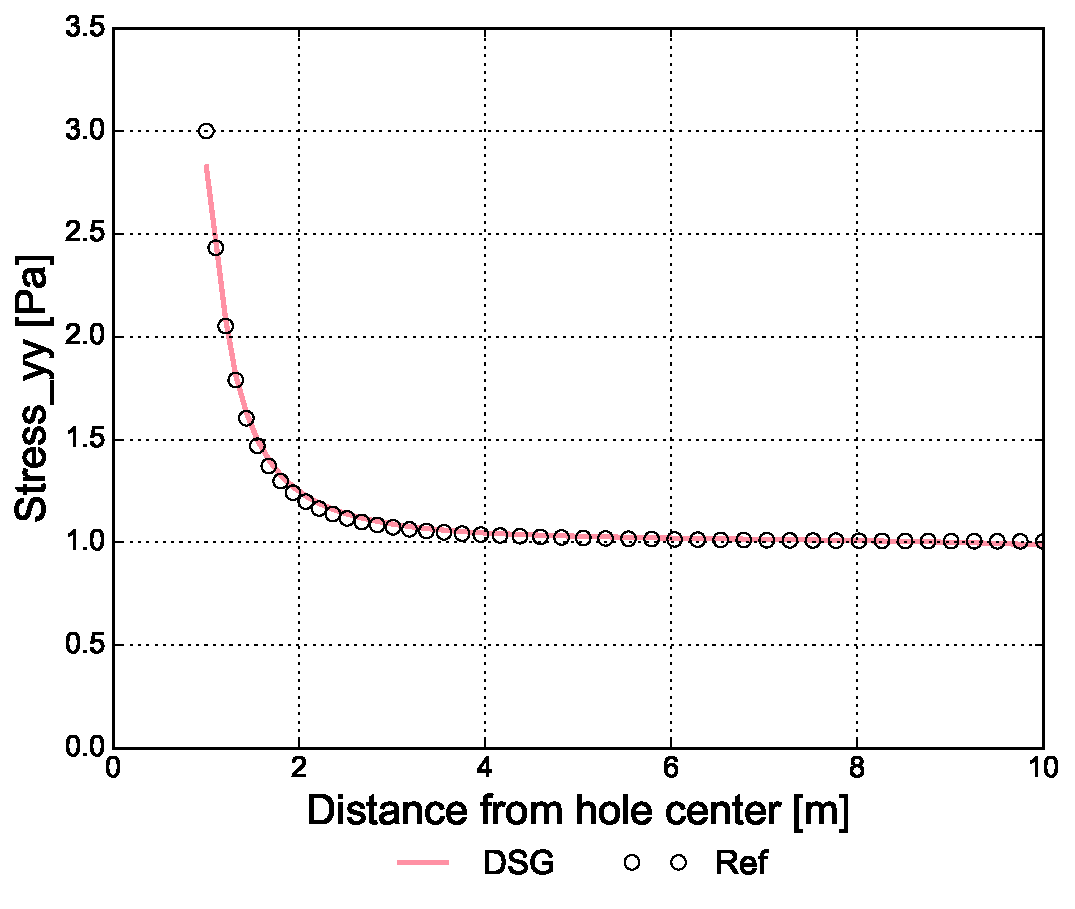
\includegraphics[width=7.3cm]
		{plate_with_hole_results.pdf}}
	\caption{\label{Oscillating clamped plate benchmark}LEFM stress concentration factor benchmark}
\end{figure}

asdf